\section{Semantic Parsing}
\label{cap2:theoFrame/semPar}
As mentioned by Kamath and Das~\cite{semPar:KamathD19}, Semantic Parsing is defined as the 
mapping from a natural language utterance into a semantic representation. These 
representations usually refer to logical forms, meaning representations or programs, which 
are executed over an underlying context such as relational tables or Knowledge Graphs. This 
execution yields a desired output like an answer to a question. For example, given a question 
in natural language, a semantic parser can aim to generate a valid \SPARQL{} query based on the 
Wikidata’s ontology grammar that produces the correct answer when executed over a Wikidata 
endpoint.

The first component of a Semantic Parsing framework is the \textbf{language} to represent 
logical forms or meaning representations such as logic based 
formalisms~\cite{semPar:LiangBLFL16,semPar:ArtziFZ13}, graph based 
formalisms~\cite{semPar:BanarescuBCGGHK13,semPar:OepenKMZCFHU15} or programming 
languages~\cite{semPar:FeurerKESBH15}. In particular, we focus on query languages such as \SQL{} 
or \SPARQL{}. Another component is the \textbf{grammar}, which is a set of rules used to decide the 
expressivity of a semantic parser. An example is the Combinatory Categorial Grammar for complex 
structured queries~\cite{semPar:steedman1996}. A last component is the \textbf{underlying context}, 
which is the environment over which the output mappings are interpreted or executed. Knowledge 
Graphs such as Wikidata or DBpedia serve as examples of an underlying context.

The early attempts for Semantic Parsing were systems based on rules or statistical techniques. 
Among the rule-based systems, systems could be based on pattern matching~\cite{semPar:Johnson84a} 
or syntax-based systems~\cite{semPar:Woods73}. Though their implementation is simple, 
rule-based systems tend to be domain specific, thus hard to adapt to other domains. On the 
other hand, statistical models are able to train given examples of input-output pairs from 
any domain. Many approaches require a lexicon as a-priori 
knowledge~\cite{semPar:ZelleM96, semPar:ThompsonM03}, which is used to extract relevant 
semantic or syntactic information. Since these examples are usually manually annotated or 
require complex annotations, statistical models are hard to scale. There is also an issue 
with data sparsity, so these models only work in narrow domains.

Some of the most recent approaches that have emerged are based on Sequence-to-Sequence (Seq2seq) 
models, which usually uses an encoder-decoder framework based on neural networks. Some 
approaches implement an end-to-end paradigm where an intermediate representation is not 
needed to deliver a meaning representation; thus they do not rely on lexicons, templates or 
manually generated features. Though traditional approaches are able to better model and 
leverage the in-built knowledge of logic compositionality, approaches based on sequence 
models outperform traditional approaches due to the fact that Seq2seq-based models generalize 
better with more complex and longer sentences~\cite{semPar:JiaL16}. Furthermore, Seq2seq-based 
models can also generalize across domains~\cite{semPar:KamathD19}.

In the following subsections, we discuss in more depth how systems based on 
Sequence-to-Sequence models work. First, we will briefly explain Sequence-to-Sequence models 
along with the approach we will use in this work: the Convolutional Sequence-to-Sequence model. 
Then, we will introduce Neural Machine Translation systems and how these models can be used 
for the task of translating natural language questions to \SPARQL{} queries.

\subsection{Sequence to Sequence models}
\label{cap2:theoFrame/semPar/seq2seq}
The Sequence-to-Sequence (Seq2seq) model was first introduced by 
Cho et al.~\cite{seqlab:ChoMBB14} for statistical Machine Translation. 
They proposed a neural network model based on an encoder-decoder framework 
which is based on recurrent neural networks 
(RNNs)~\cite{semPar:werbos1990, semPar:rumelhart1986,seqlab:HochreiterS97}. More details 
about RNNs can be found in Appendix~\ref{appendix:neuralNetworks}.

In a Seq2seq architecture, the encoder converts a variable-length sequence into a fixed-length 
vector representation (i.e., it encodes the input sequence into a context vector) which is 
passed through to the decoder that transforms this fixed-length vector representation back 
into a variable-length sequence (i.e. decodes a context vector back to another output 
sequence). Figure~\ref{fig:seq2seqModel} illustrates graphically how a Seq2seq looks, where 
the length $T$ of the input sequence does not necessarily equal the length $T'$ of the output 
sequence.

\begin{figure}[!h]
    \centering
    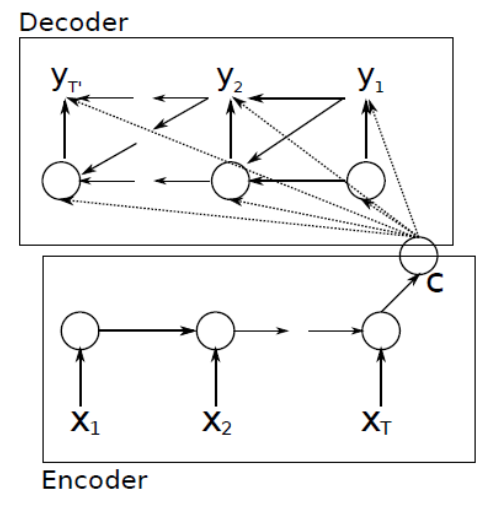
\includegraphics[scale=.5]{imagenes/2_theorical_framework/semantic_parsing/seq2seqModel.PNG}
    \caption{Sequence to Sequence model~\cite{seqlab:Graves2012-385}.}
    \label{fig:seq2seqModel}
\end{figure}

Technically, the model is learning a conditional distribution over a variable-length sequence 
conditioned on yet another variable-length sequence $p(y_1,\ldots,y_T'|x_1,\ldots,x_T)$. The 
encoder is an RNN that reads each symbol of an input sequence $x$ sequentially. While it is 
reading the current symbol on each step $t$, the hidden state $h_{t}^e$ of the RNN changes are
described as:

\[
    h_{t}^e= f(h_{t-1}^e,x_t)
\]

After reading the end of the sequence, the hidden state of the RNN is the summary $c$ of the 
whole input sequence, also known as its context vector. Then, the decoder is another RNN 
trained to generate the output sequence by predicting the next symbol $y_t$ given the hidden 
state $h_{t}^d$. This prediction is also conditioned on the previous predicted symbol 
$y_{t-1}$ and on the context vector $c$. Then, the hidden state of the decoder is defined 
for the step $t$, where $f$ is usually the \textit{sigmoid} function:

\[
    h_{t}^d= f(h_{t-1}^d,y_{t-1},c)
\]

Similarly, the conditional distribution of the next symbol, where $g$ is commonly a 
\textit{softmax} function since a valid probability must be produced, is defined as follows:

\[
    P(y_t|y_{t-1},y_{t-2},\ldots,y_1,c) = g(h_{t-1}^d,y_{t-1},c)
\]

Both components of the sequence model are jointly trained to maximize the following 
conditional log-likelihood function:

\[
    max_{\theta} \: \frac{1}{N} \sum_{n=1}^N log \; p(y_n|x_n)
\]

Once the model is trained, it can be used to generate a target sequence given an input 
sequence. Though Seq2seq models were originally designed based on RNNs, other variants have 
emerged~\cite{semPar:SutskeverVL14,nmt:DongL16}; among the more modern ones, a recent work 
introduces a sequence learning approach based on convolutional neural networks, which has 
shown to outperform many RNN-based models in the task of \NLtoSPARQL~\cite{nmt:nl-to-sparql-Yin19}.

\subsubsection{Convolutional Sequence to Sequence Model}
\label{cap2:theoFrame/semPar/seq2seq/convS2S}
A Seq2seq model based completely on convolutional neural networks (CNNs) is 
proposed by Gehring et al.~\cite{nmt:convS2S-GehringAGYD17}, called the Convolutional 
Sequence-to-Sequence model (ConvS2S). For this subsection we will assume a basic 
understanding of CNNs, where more details about this topic can be found in 
Appendix~\ref{appendix:neuralNetworks}.

Since CNNs do not receive the input as a sequence like RNNs do, a \textbf{position embedding} 
is proposed. First, the input elements $x=(x_1,\ldots,x_m)$ are embedded in distributional 
space as $w=(w_1,\ldots,w_m)$, where $w_j$ is a column in an embedding matrix $D$. These 
embeddings are combined with an absolute position vector $p=(p_1,\ldots, p_m)$, which 
indicates the position of the word in the sequence, in order to establish a sense of order in 
the input. From this combination the input element representation $e=(w_1+p_1,\ldots, w_m+p_m)$ 
is obtained. The output elements generated by the decoder are built using a similar 
representation.

To compute intermediate states, a simple \textbf{convolutional block structure} is used for both 
encoder and decoder, where such blocks are also referred to as \textit{layers}. These intermediate 
states are based on a fixed number of input elements whose output for the l-th block are 
denoted as $z^l=(z_1^l,\ldots,z_m^l)$ for the encoder network and $h^l=(h_1^l,\ldots,h_m^l)$ 
for the decoder network. Each block contains a one dimensional convolution followed by a 
non-linearity.

Each convolution kernel is parameterized as $(W, b_w)$ and takes as input $X$, which is a 
concatenation of $k$ input elements embedded in $d$ dimensions, and maps them to a single 
output element $Y$. Subsequent blocks operate over the $k$ output elements of the previous 
block. The gated linear unit (GLU)~\cite{semPar:DauphinFAG16} was chosen as the non-linearity 
to apply over the output of the convolution $Y$. This gating mechanism permits to control which 
input values of the current context are relevant. Aside from that, to enable deep convolutional 
networks, residual connections are added from the input of each convolution to the output of the 
block~\cite{semPar:HeZRS15}.

The input of the encoder network is padded to match the output length of the convolutional 
blocks for each block. The padding is done by adding $k - 1$ zero vectors on both the left 
and right side of the input to then remove k elements from the end of the convolution output. 
The same padding cannot be done for the decoder network since no future information is known 
beforehand~\cite{semPar:OordKK16}.

A linear mapping is added for projecting between the embedding size and the convolution 
outputs. This mapping is applied to $w$ when feeding embeddings to the encoder network, to the 
encoder output $z_j^u$, to the final block of the decoder just before the softmax $h^L$, and 
to all decoder blocks $h^l$ before computing the attention score, which is explained later. 

Lastly, a distribution is calculated over the $T$ possible next target elements $y_{i+1}$ by 
transforming the top decoder output $h_i^L$ via a linear layer with weights $W_o$ and bias 
$b_o$, as follows:

\[
    p(y_{i+1}|y_1,\ldots,y_i,x)=softmax(W_o h_i^L + b_o)
\]

Besides the convolutional block structures, a separate \textbf{attention mechanism} is implemented 
for each decoder layer. Attention allows the model to focus on the relevant parts of the 
sentence for each time step. The entire process is illustrated in 
Figure~\ref{fig:convBlockStruct}. The calculation of the attention starts in the bottom left 
part of Figure~\ref{fig:convBlockStruct} with a combination between the current decoder state 
$h_i^l$ and the embedding of the previous target element $g_i$, which is defined as:

\[
    d_i^l= W_d^l h_i^l + b_d^l + g_i
\]

Then looking at the center part of Figure~\ref{fig:convBlockStruct}, for a decoder block $l$, 
the attention $a_{ij}^l$ of state $i$ and source element $j$ is computed as a dot-product 
between the decoder state summary $d_i^l$ and each output $z_j^u$ of the last encoder block $u$:

\[
    a_{ij}^l = \frac{exp(d_i^l \cdot z_j^u)}{\sum_{i=1}^m exp(d_i^l \cdot z_j^u)}
\]

Subsequently, the conditional input $c_i^l$ to the current decoder block is a weighted sum of 
the encoder outputs as well as the input element embeddings $e_j = w_j + p_j$ which corresponds 
to the center right part of Figure~\ref{fig:convBlockStruct}, and is defined as:

\[
    c_i^l = \sum_{j=1}^m a_{ij}^l (z_j^u + e_j)
\]

Finally, the conditional input $c_i^l$ is added to the output of the corresponding decoder layer 
$h_i^l$, as seen in the bottom right part of Figure~\ref{fig:convBlockStruct}. Compared with the 
classical single step attention, this proposal is named a \textit{multi-step attention} mechanism 
since each step takes into account the attention history of the previous time steps, based on how 
conditional inputs are computed. Thus, information does not struggle to survive several steps 
as happens with recurrent networks.

\begin{figure}[!h]
    \centering
    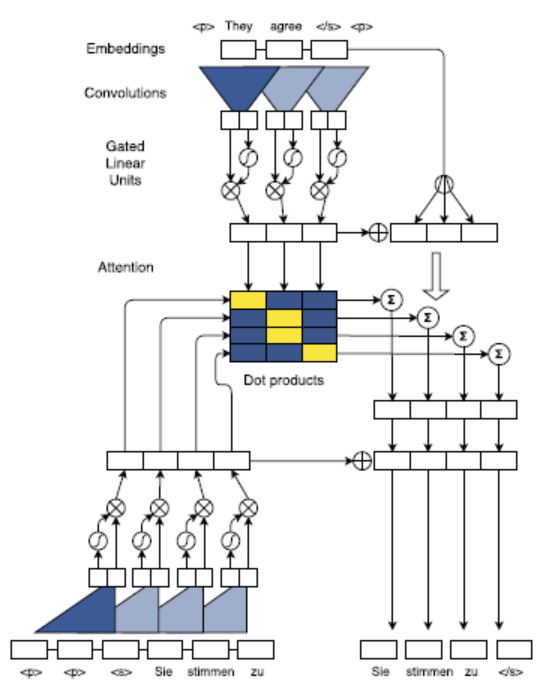
\includegraphics[scale=.5]{imagenes/2_theorical_framework/semantic_parsing/conS2SModel.PNG}
    \caption{Convolutional block structure with a multi-step attention mechanism~\cite{nmt:convS2S-GehringAGYD17}.}
    \label{fig:convBlockStruct}
\end{figure}

Some \textbf{normalization strategies} are applied to stabilize the learning process. First, 
the input and output of a residual block are summed with $\sqrt{0.5}$ to halve the variance of 
the sum. Second, the conditional input $c_i^l$ are scaled by $m\sqrt{1/m}$ to counteract any 
change in variance. Lastly, for convolutional decoders with multiple attention, the gradients 
for the encoder blocks were scaled by the number of attention mechanisms used, excluding source 
word embeddings.

Besides scaling, a \textbf{weight initialization} is also done to keep variance retained. 
Embeddings are initialized from a normal distribution with mean 0 and standard deviation 0.1. 
Weights from layers whose output is not directly fed to a GLU are initialized from 
$\mathcal{N}(0, \sqrt{1/n_l})$, where $n_l$ is the number of input connections to each neuron. 
This helps to maintain a variance of the input with a normalized distribution. Layers followed 
by a GLU are initialized from $\mathcal{N}(0, \sqrt{4/n_l})$, which is a weight initialization 
scheme based on works by He et al.~\cite{semPar:HeZRS15} and Glorot \& Bengio~\cite{semPar:GlorotB10}. 
Biases are uniformly set to zero. Lastly, dropout is applied to the input on some layers with a 
probability of p of being retained and so scaled by $1/p$, or setting them to zero 
otherwise~\cite{semPar:SutskeverVL14}.

\subsection{Natural Language to SPARQL}
\label{cap2:theoFrame/semPar/nlToSparql}
Though most works have focused on translating natural language to \SQL{} queries~\cite{nmt:CaiXZYLL18,nmt:ZhongCoRR17}, 
recent work has also addressed the translation of natural language to \SPARQL{}. In particular, 
Neural Machine Translation (NMT), which involves Machine Translation systems based on Neural 
Networks, has been used to develop systems that translate questions to \SPARQL{} queries. An 
evaluation of eight different NMT models was performed by Yin et al.~\cite{nmt:nl-to-sparql-Yin19}. 
The NMT models included in this work were based on the aforementioned encoder-decoder Seq2seq 
architecture. Among these models, six of them are based on recurrent neural networks (RNN), 
while the remaining two are based on the ConvS2S model~\cite{nmt:convS2S-GehringAGYD17} and 
the Transformer model~\cite{semPar:VaswaniSPUJGKP17} respectively.

The systems based on RNNs include a baseline and many variants of the same LSTM architecture 
and different types of attention mechanisms. As a baseline, a Neural SPARQL Machine 
(NSpM)~\cite{nmt:nspm-SoruMMPVEN17, nmt:CoRRSoru18} is used, which consists of a 2-layer LSTM 
model with no attention mechanisms. Then, two variants of the NSpM are used with two different 
types of attention: global attention and local attention. Global attention uses the entire 
input sentence to calculate an attention vector, which complements the context vector output by 
the encoder~\cite{nlToSparql:BahdanauCB14}. On the other hand, local attention only uses a 
fixed size window around every word of the sequence to calculate a scoped attention vector per 
word~\cite{nlToSparql:LuongPM15}. Another model is based on a proposal from 
Luong et al.~\cite{nlToSparql:LuongPM15}, which consists of a 4-layer LSTM model with local 
attention. Lastly, the Google Machine Translation (GNMT) architecture~\cite{nlToSparql:WuSCLNMKCGMKSJL16} 
is included with two different variants: a 4-layer LSTM and a 8-layer LSTM, both with local 
attention. The only difference between Luong’s model and the GNMT is that the second model 
includes residual connections from the third layer and uses a bidirectional LSTM in the first 
layer of the encoder.

\subsubsection{Neural Machine Translation}
\label{cap2:theoFrame/semPar/nlToSparql/nmt}
Though the architecture of each model varies, the encoding of \SPARQL{} queries used in all 
approaches is the same as that proposed by Soru et al.~\cite{nmt:nspm-SoruMMPVEN17}. Their 
encoding suggests that URIs are abbreviated using their prefixes  followed by an underscore; 
brackets and dots are replaced by their verbal description, and \SPARQL{} keywords are lower-cased. 
For example, a query over Wikidata is shown in Listing~\ref{lst:decodedWikidataSparqlExample}, 
when after an encoding conversion, it is converted to an encoded query as seen in 
Listing~\ref{lst:encodedWikidataSparqlExample}.

\begin{sparqlcode}[%
    caption={\SPARQL{} query before encoding.}, 
    label={lst:decodedWikidataSparqlExample}]
PREFIX wd: <http://wikidata.org/wiki/>
PREFIX wdt: <http://wikidata.org/prop/direct/>

SELECT ?sbj 
WHERE {
    ?sbj wdt:P19 wd:Q201007 .
    ?sbj wdt:P166 wd:Q37922 .
}
\end{sparqlcode}

After training, the system will output an encoded form that can be transformed back to the 
original \SPARQL{} representation. 

\begin{sparqlcode}[%
    caption={\SPARQL{} query after encoding (note it excludes the \texttt{PREFIX} clauses).}, 
    label={lst:encodedWikidataSparqlExample}]
select var_sbj where brack_open var_sbj wdt_p19 wd_q201007 sep_dot var_sbj wdt_p166 wd_q37922 sep_dot brack_close
\end{sparqlcode}

The evaluation metrics typically used to compare these systems are string-matching Accuracy, 
BLEU score and Perplexity. The string-matching Accuracy is used to measure the amount of exact 
matches delivered by each system. The global Accuracy is then the percentage of cases that are 
syntactically equal to the expected answer. This metric is particularly useful when measured 
over a dataset based on \SPARQL{} templates, giving insights into whether or not the expected 
\SPARQL{} form is being correctly generated.

The Bilingual Evaluation Understudy (BLEU) score is used to measure how similar two sentences 
are by using a geometric average of modified n-gram Precision~\cite{nlToSparql:PapineniRWZ02}, 
which is represented by the following formula:

\[
    BLEU = BP \cdot exp(\sum_{n=1}^N w_n \; log \: p_n)    
\]

The modified Precision $p_n$ for each candidate counts the number of times an n-gram occurs in a 
reference translation(s), takes the maximum count of each n-gram among the reference(s), and 
then clips the count of each n-gram in the candidate translation to the maximum count. To avoid 
short candidate translations getting higher scores than desired, a brevity penalty (BP) is 
applied which is set to 1 if the candidate length $c$ is larger than the maximal reference 
length $r$ or set to $exp(1-r/c)$ otherwise. The $w_n$ represents weights for each modified 
Precision. By default $w_n=\frac{1}{N}$ and $N=4$. In this case, the BLEU score goes from 0 to 
100, where a score closer to 100 means the model is performing better. Note that BLEU does not 
account for word order. 

\textbf{Perplexity} is used to understand the model’s intrinsic behavior based on a cross 
entropy H(p,q) which is defined as follows:

\[
    H(p,q)= -\sum_x p(x) \; log \: q(x)
\]

\noindent where $p$ represents the target probability distribution and q is the estimated probability 
distribution. Their similarity is defined by all possible values $x$ in the distribution. In 
this case, $p$ is the one-hot encoding vector of the target vocabulary and q is deduced from 
the result of the output softmax layer. Then the Perplexity is defined as the exponentiation 
of the cross entropy:
\[
    perplexity(p,q)=2^{H(p,q)}
\]

According to the experiments conducted by Ying et al.~\cite{nmt:nl-to-sparql-Yin19}, the model 
that performs best was the ConvS2S model. Although many datasets were used in their experiments, 
we are only interested in \LCQuADone~\cite{dataset:lcquad2-DubeyBA019} and 
\DBNQA~\cite{dataset:dbnqa-hartmann-marx-soru-2018}, two datasets that represent opposite traits 
of a Question Answering Dataset: the \LCQuADone{} dataset contains few questions (5000) but with high 
complexity and high variance of its questions while the \DBNQA{} dataset contains a huge volume of 
questions (nearly $900,000$) but it lacks variety in its questions. We explain with more details 
what we understand by a \dquotes{good dataset} in the \textit{Question Answering} section~\ref{cap2:theoFrame/qakg}. 
The results of the three best models among the eight selected over the mentioned datasets are 
shown in Table~\ref{table:nmtYinResults}.

\begin{table}[h!]
    \centering
    \resizebox{\textwidth}{!}{%
    \begin{tabular}{|l|ll|ll|ll|ll|ll|ll|}
    \hline
    \multirow{2}{*}{} & \multicolumn{4}{c|}{\textbf{Perplexity}}                                                                    & \multicolumn{4}{c|}{\textbf{BLEU Score}}                                                                  & \multicolumn{4}{c|}{\textbf{Accuracy}}                                                                    \\ \cline{2-13} 
                      & \multicolumn{2}{c|}{\textbf{LC-QuAD 1}}              & \multicolumn{2}{c|}{\textbf{DBNQA}}                  & \multicolumn{2}{c|}{\textbf{LC-QuAD 1}}             & \multicolumn{2}{c|}{\textbf{DBNQA}}                 & \multicolumn{2}{c|}{\textbf{LC-QuAD 1}}             & \multicolumn{2}{c|}{\textbf{DBNQA}}                 \\ \hline
    \textbf{Models}   & \multicolumn{1}{l|}{\textbf{Train}} & \textbf{Valid} & \multicolumn{1}{l|}{\textbf{Train}} & \textbf{Valid} & \multicolumn{1}{l|}{\textbf{Valid}} & \textbf{Test} & \multicolumn{1}{l|}{\textbf{Valid}} & \textbf{Test} & \multicolumn{1}{l|}{\textbf{Valid}} & \textbf{Test} & \multicolumn{1}{l|}{\textbf{Valid}} & \textbf{Test} \\ \hline
    LSTM\_Luong       & 1.12                                & 4.92           & 1.90                                 & 2.15           & 52.43                               & 51.06         & 77.64                               & 77.67         & 0                                   & 0             & 34                                  & 34            \\
    ConvS2S           & 1.14                                & 3.25           & 1.12                                & 1.25           & 61.89                               & 59.54         & 96.05                               & 96.07         & 8                                   & 8             & 85                                  & 85            \\
    Transformer       & 1.16                                & 3.15           & 2.21                                & 3.34           & 58.99                               & 57.43         & 68.68                               & 68.82         & 7                                   & 4             & 3                                   & 3             \\ \hline
    \end{tabular}%
    }
    \caption{Performance comparison of three models included in Yin et al.\cite{nmt:nl-to-sparql-Yin19}.}
    \label{table:nmtYinResults}
    \end{table}

Based on the Perplexity results, there is a serious overfit for all models over the \LCQuADone{} 
dataset which Yin et al. attributes to the small size of the dataset and its complex questions. 
No evident overfit is spotted over \DBNQA, and the ConvS2S shows better results which is 
reflected in the other results as well. The BLEU score results reflect that ConS2S again 
outperformed all other models and shows a correlation between Perplexity and BLEU, especially 
when looking at \DBNQA{} results. Finally, Accuracy results clearly show that RNN based models and 
the Transformer do not perform positively in any case when compared to the ConvS2S model. 
However, the results over the \LCQuADone{} dataset shows there is still a challenge regarding 
the handling of more complex questions among all NMT models.

